%\typeout{-------------------------------------------------}
%\typeout{Macros redefined and reloaded in fsm.tex}
%\typeout{remember to remove them when you include bugs.tex}
%\typeout{-------------------------------------------------}
%\input totals.tex
%\newcommand{\anarrow}{\(\Rightarrow\)}
%%%%%%%%%%%%%

\chapter[A connectionist model of multicolumn arithmetic]{A
Connectionist Model\\of Multicolumn Arithmetic}\label{c:fsm}

Before detailing the connectionist network used to model
arithmetic, this chapter first outlines the known features of arithmetic
that constrain the model.
The architecture, input and output
representations and training environment are then described.  The results
of simulations---the errors the network makes when solving multicolumn
problems---are presented, and the network's behaviour is
analysed.  Finally there is a discussion of how the network relates to
Sierra, and how notions like bug migration and impasses can be
accommodated.


\section{Constraints on the model}

Few people do long multiplication ``in the head'', preferring instead to
use an external representation on paper.  This kind of mundane
observation needs to be incorporated into the design of any model in order
to constrain it.  These constraints are listed in this section.

One thing which is {\em not\/} constrained is the grain size of the model,
yet this is often what makes or breaks a model.  Choosing the wrong
set of operators can mean that the model apparently fails in its task.  An
example of this is VanLehn's decision to include ``leftmost column'' as
part of the problem representation; without it Sierra would not be able to
account for the bug always-borrows-left (figure~\ref{f:abl}). Of course,
empirical validity is not the only measure of a model (as discussed on
page~\pageref{p:empirical}), but without a reasonable fit to the data it
becomes difficult to judge the explanatory power of a model.  These issues
are taken up throughout this chapter.

\subsection{What we know about multicolumn arithmetic}

Taking assumptions and observations from
\citeA{mindbugs} and \citeA{younerro}, it is possible to present a list of
some of the things that are known about arithmetic:

\heading {Children don't understand it} This point was discussed at length
in section~\ref{s:sierra}, concluding that multicolumn arithmetic is best
described in terms of a procedural (syntax-only) set of skills.

\heading {It takes time} Many connectionist models solve whole problems in
a single step: input is presented, and an output is computed.  Multicolumn
arithmetic, however, is characterized by its sequential nature.  A network
in this domain must be able to produce a series of actions even when the
external input does not change.

\heading {Problems vary in length} There is no point in building a network
which can only solve problems containing a limited number of digits.  The
power of multicolumn arithmetic stems from the fact that a simple set of
arithmetic procedures can be applied to problems of unlimited length.  This
point and the previous one are the main reasons for selecting a {\em
recurrent\/} network as the architecture of the model.

\heading {There are eye movements} \citeA{suppproc} measured the eye
movements made by subjects when solving multicolumn arithmetic
problems.  It was showed that subjects tend to follow the
normative algorithms taught in schools. That is, for addition the eye
focusses
at the top of the page, scans down the column, then jumps to the start of
the next column, and so on. This information was used by
\citeauthor{suppproc}\ to build a model of eye movements (discussed later).
Eye movements are not accounted for in the symbolic models of buggy
arithmetic.  In the \citeauthor{younerro} account the operation
\verb|ReadMandS| deposits the digits of the current column into the working
memory; the operations \verb|ShiftLeft| moves attention to the next column.
Hence eye movements are below the level of detail addressed by the current
symbolic accounts.

\heading {You don't always mark the page} The subject is not marking the
page when focussing on a digit, or recalling the product of a
multiplication. Again this can be viewed as a question of grain size: It is
possible to build a model in which each operation is quite complex,
resulting in a mark being made on the page, although no existing models
suggest such a coarse level of detail.  Given the serial scanning nature of
arithmetic, the model described in this chapter includes a simple form
of eye
movement, whereby a focus of attention is shifted digit by digit over the
problem.  Each step does not necessarily mark the page, which means that
the network will have to rely on some kind of internal memory to know what
to do when the input does not change.

\heading {Arithmetic is learned in steps} Many connectionist networks are
trained by presenting the system with a broad set of instances from a
target mapping.  As described in section~\ref{s:sierra} there is a definite
curriculum for arithmetic. This means the training set for the model will
be ``staged''.  First the network will be trained on simple addition
problems involving just two
digits with no carrying.  Then, two column problems are
introduced and trained along with the previously learned problems
\cite<to avoid catastrophic interference; see>{mcclcata,ratcconn,mcracata}.
It is not the case that staged learning makes this problem easier to learn
\cite<as it did for>{elmaincr}.  Rather, the network described below will
learn the training set three or four times faster when the
problems are presented in a single training set. The cost of this speed-up
is that the bugs exhibited by such a network include such unlikely actions as
carrying on simple problems like 1+1. It could be argued that, early in
learning, children solving 1+1 would not
have the concept of carrying, hence such errors are never going to be
observed.  So to avoid such star bugs, and to mimic the training
environment of children, the input to the network is staged.

\heading {Learning is by example, not verbal recipes} This was discussed
in section~\ref{s:sierra}.  This is convenient for a connectionist model
because it means the system can be trained from actual example problems,
rather than trying to get a network to (somehow) interpret an encoding of
the procedures for arithmetic.

\heading {There are bugs and slips}  Run time slips, such as \x34=8, were
considered in part~\ref{c:mental}.  Here the focus is on procedural
misconceptions, where mistakes are not due to ``faulty recall'', but result
from mislearning.  To isolate the procedural aspects of arithmetic, much
of the processing involved in solving a
problem is done outside the network.  External activities include
keeping track of the current focus of attention, computing products,
and keeping running totals. Training
a network to output the right steps in a procedure (``multiply now'',
``remember this number'') is hard enough without all the additional details
of register storage, and remembering the multiplication facts.  The result
is a connectionist finite state machine.  Embedding the facts
network from chapter~\ref{c:xnet} inside this state
machine would be an interesting project, but it is not taken up here.

\heading {Bugs occur during testing} Many bugs show themselves when the
subject attempts to solve previously unseen problems (see
section~\ref{s:emprical}).  After training a network on a set of problems,
any over-generalization can be assessed by presenting a test set of slightly
harder problems---namely the next set of problems in the curriculum
sequence. In some circumstances it may be possible to find a training set
that leads to near-perfect generalization. With this in mind
\citeA{vanltwo} discusses the notion of a pseudo-student---a program that
will take a textbook lesson sequence and return a list of the
misconceptions students are likely to acquire from that particular set of
problems. Using this knowledge it will be possible to adjust the textbook's
lessons to reduce the likelihood of students acquiring misconceptions.

Many of the assumptions of the model are based around the assumptions of
VanLehn's theory.  Others may disagree with these assumptions, for example
about learning being from examples only. However, to give this domain a
connectionist treatment, it seems sensible to start from the assumptions of
an established theory, rather than attempt to reconstruct a new one.

\subsection{What we don't know about multicolumn arithmetic}

The above points help to narrow down the design of a model, but there
are a number of fundamental questions which throw the design space wide
open. Three particular unknowns are:

\heading {What is read} Although the eyes move this does not mean we
know what is actually read from the page.  Do subjects just look at
single digits, or is the context of the digit, such as the space
around it, important?  Reading
arithmetic problems is nothing like reading text: \citeA{suppread} found
that two, quite different models were needed to capture eye movements in
these two domains.

\heading {What is done} In terms of virtual machines, what are the
operations carried out on an arithmetic problem?  This is not just a
problem of getting the right grain size, but of getting an appropriate set
of operations, as discussed at the start of this section.  Given that
there are many instruction sets that can perform a given task, what are the
criteria for favouring one over another? With enough degrees of freedom it
is always possible to produce a fit to the data, so empirical adequacy is
only part of the story.

\heading {How we navigate problems} What kind of cues does a subject use
when solving a problem?  When looking for the top of a column, does the eye
scan up until it finds a large enough area of space? Or is there some kind
of peripheral information allowing a fast, ballistic movement?


These unknowns are mostly ignored in all the accounts of arithmetic
malrules to date.  What is missing is a solid understanding of the
perceptual processes underlying our symbolic arithmetic abilities. As
\citeA{suppproc} comment: ``Without such a [perceptual] component we have
no way of representing the mental operations a person actually uses to
process the written symbols presented to him'' (p.~342).  Given the lack of
empirical research in this area, I have used many of the detail from the
work of \citeauthor{suppproc}\ to design the connectionist model.


\begin{fancyfigure}
\centerline{\psfig{file=addtrans.ps,width=11cm}}
\caption{Transition network for long addition based on routines by
\protect\citeA{suppproc}.  Digits in the problem are represented in a
coordinate system (row,column), relative to a top-right origin (1,1).
A movement is denoted ($\pm$ row,$\pm$ column).
Subprocedures are used for
vertically scanning a column.}
\label{f:addtrans}
\end{fancyfigure}


\subsubsection{The \protect\citeauthor{suppproc}\ model of eye movements}

The register machine presented by
\citeA{suppproc} was built to capture
eye-fixation durations and saccade directions for multicolumn addition
and subtraction. In particular the aim was to ensure that eye movements
could be correlated to steps in the register machine. The model's
operations included:
\begin{itemize}
\item A stimulus supported register (SS) which contains the element
(digit, rule mark, space) currently being looked at. The SS register is
subject to decay when the focus of attention is moved.
\item A nonstimulus-supported register (NSS), which is not subject to
decay.  This register is used to accumulate an answer.
\item A copy operation allows the contents of SS to be moved to NSS.
\item The left- or right-most digit of a register can be written out.
For two digit numbers this obviously means having access
to the tens and units of the number.
\item Arithmetic facts are supplied by a ``lookup'' operation.
\item Conditional branch points are used---``gotos'' which are dependent
upon the contents of a register.
\item The problem is represented as cells in a grid.
\item The focus of attention is directed by an ``attend'' operation,
which is either absolute (attend to grid position $a,b$), or relative
(shift attention by $\pm a,\pm b$).
\end{itemize}

Using these elements, \citeauthor{suppproc}\ found that a register model
could be built in which the operations correlated with eye activity
(figure~\ref{f:addtrans}).
That is, eyes tend to move when the register machine requires movements
(attend), and stay put during other cycles (copy, lookup, etc.). Of course,
eye movements are highly stochastic, and the measures of correlation that
\citeauthor{suppproc}\
used are necessarily complex.  Despite the success of
the model there are many more aspects to consider---e.g., the
use of the grid system of coordinates, and eye movement velocities.

The basic elements from this model of arithmetic eye movements were used as
the starting point for the connectionist model described in the next
section. Although \citeauthor{suppproc}\
did not attempt to model arithmetic
malrules, their analysis of of the perceptual systems should be an
important component of any arithmetic model.


%%%%%%%%%%%%%%%%%%%%%%%%%%%%%%%%%%%%%%%%%%%%%%%%%%%%%%%%%%%%%%%%%%%%%%%%%%%

\begin{fancyfigure}
\centerline{\psfig{file=longxnet2.ps}}
\caption{Architecture of the model. Outputs from the network drive
external machinery (ALU) to perform tasks such as addition and
multiplication.}
\label{f:longnet}
\end{fancyfigure}
\section{Architecture of the model}

Having looked at the origins of the ideas behind the connectionist model,
it is now
possible to specify the details.  The architecture
is shown in figure~\ref{f:longnet}.  An encoding of the problem is
presented to a recurrent network, which activates a set of 35 hidden units,
which in turn activates an output layer representing actions to be carried
out.  These actions drive external mechanisms to update the problem in
various ways, such as writing down a number, moving the focus of attention,
or computing a sum or product.  To enable the network to process
sequences, the hidden layer is copied to the context layer at each time
step acting as a memory of the previous state.

We can view the problem of learning arithmetic algorithms as learning to be
a finite state machine (FSM). \citeA{mindbugs} also
found it useful to describe long subtraction in terms of transition
networks.

There are plenty of connectionist models that can learn to be FSMs
\cite{pdp:8,elmafind,servenco,cottlear,clues,willexpe,rcascor}. I chose to
use backpropagation through time (BPTT), as proposed by
\citeA[pp.~354--361]{pdp:8}.  BPTT involves stacking-up a copy of a
feedforward network for each step in a sequence, and then ``rewinding'' at
the end of the sequence, backpropagating error to the very first pattern in
the sequence. Although it seems to be an unpopular algorithm, it has
distinct advantages over other candidates: it can learn sequences that
simple recurrent networks find difficult \cite{maskforc}; it shows better
performance, in terms of generalization
and learning success, that the real-time
recurrent
learning algorithm \cite{zipssubg};
and backpropagation is better understood than
more recent constructive algorithms, such as cascade correlation.

\begin{fancyfigure}
\centerline{\psfig{file=bptt.ps,height=7cm}}
\caption{Backpropagation through time (BPTT). The shaded area shows a
single network.  I(t) is the input at a particular time step, t. H
represents a hidden layer, and O represents an output layer. The training
of a recurrent net is reduced to training a many-layered feed-forward
network.}
\label{f:bptt}
\end{fancyfigure}

BPTT works by making one copy of the network for each step in the problem.
As the context layer is the hidden layer from the previous time step, it is
possible to re-draw a BPTT network as in figure~\ref{f:bptt}.  At each step
of the forward pass, the activations of all the layers are recorded.
 After the last output has been
produced, error is backpropagated down the virtual network in the usual
way.  In the figure, error is propagated from O(2) to H(2), allowing
error information to be computed from H(2) to H(1).  Also, at this point
O(1) contributes the error associated with the output at time step 1.
This continues with
H(1) backpropagating error to H(0), and so on.  Note that the weights from
I(1) and H(0) to H(1) and O(0), are exactly the same as the weights from
I(2) and H(1) to H(2) and O(1).  After the error has been backpropagated to
the start of the network, the weights are updated using the generalized
delta rule \cite{pdp:8}.

The BPTT algorithm differs from the use of backpropagation in
simple recurrent networks (SRNs) because error is preserved across the
hidden layers.  SRNs \cite<as described by>{elmafind} have the feed back
from the hidden layer to the context layer, but do not stack up copies of
the network.  Error is computed after each pattern.  When using a near
minimal number of hidden units for a task, SRNs can carry information about
certain contingencies over a number of time steps. That is,
SRNs can use knowledge from previous time steps to influence actions much
later in the
sequence. ``Such information is maintained with relative ease if it is
relevant at each time step; it tends to get lost when intervening elements
do not depend on it'' \cite[p.~372]{cleefini}.  BPTT obviously does not
have this problem as the whole time sequence is drawn out.  Preliminary
tests identified that the problem of multicolumn arithmetic, as presented
here, requires BPTT\@. However, SRNs can learn this task, but only by using
many more hidden units than required \cite{maskforc}.

\begin{fancyfigure}
\centerline{\psfig{file=grammar.ps,height=5cm}}
\caption{The grammar used by \protect\citeA[p.~374]{cleefini}.
B is the designated start symbol, and E is the end symbol. Traversing an
arc generates a symbol (B,P,S,T,V,X, or E). An example string is:
BTSSSXXVVE}
\label{f:gram}
\end{fancyfigure}


\citeA{cleefini}
found that recurrent networks of this kind, when trained on
example strings from a finite state grammar, can become perfect recognizers
for that grammar \cite<see also>{servenco,servgrad,alleconn,elmafind}. A
SRN was presented with strings from an artificial grammar
(figure~\ref{f:gram}). At each time step one letter was presented, and the
network's task was to predict the next letter in the sequence.  Given that
any node in the grammar may have a number of successors, it is not possible
to correctly predict the next letter.  A particular letter's
successor will depend on the context of what other letters have been
processed---the choice of successor
will depend on which node has been reached in the
grammar.  The network was trained on 60~000 randomly selected strings from
the grammar.  When testing the network any output unit with activation
above 0.3 was taken as a prediction of a legal successor.  When the actual
successor was not one of the predicted successors, the network was said to
have rejected the string.  The string is accepted if only good
predictions have
been made when a designated terminal symbol was reached. In a test of
70~000 randomly generated strings, 0.3 per cent happened to be grammatical.
The network accepted all the grammatical strings, and rejected the others.
When the hidden unit activations were analysed, by clustering the hidden
vectors according to their similarity, it was found that the vectors
grouped according to nodes in the grammar.
% (but only when hidden unit resources are constrained).
Given that
multicolumn arithmetic can be
viewed as learning to be a FSM, it seems that this kind of recurrent
network is appropriate for the task.

\begin{fancyfigure}
\centerline{\psfig{file=eye.ps,height=6cm}}
\caption{Problem representation}
\label{f:eye}
\end{fancyfigure}

\subsection{Input and output representations}

Having selected an architecture that is powerful enough to learn arithmetic
procedures, the next step is to specify the input and output
representations.
Figure~\ref{f:eye} shows a general framework for
representing long multiplication using a grid.
To solve a problem
represented in this way requires three types of operations:
\begin{itemize}

\item Attending to particular areas of the problem to
read and write digits.  To do this the network moves a ``focus of
attention'' around the grid.

\item Computing arithmetic facts, or other useful predicates.  The
lookup of arithmetic facts is done externally to the network, and a small
number of truth values (e.g., ``in leftmost column?'') are presented as
input.

\item Controlling the attention of the network, knowing when to write
down a digit, etc.  The training set and choice of output operations
determines the control strategy.

\end{itemize}


Three external registers are used to keep track of the network's progress
through the problem.  One register is used to point to the current digit
being processed in the upper-row and another is used to point to
the digit in the second row of a problem.  These registers are not
necessary for addition, but are for multiplication.
The third register is used to locate the place
where
the answer should be written.  These registers are initialized to default
positions at the start of a problem, and it is the network's responsibility
to update them by turning on appropriate output units
associated with increment operations. When the network needs
to read the upper-row digit, the ``jump to the top row'' output unit will
be switched on.

There are may other ways that action could be represented without using
external registers. For example, the output layer could be split into an
operation-argument pair.  In this case moving the focus of attention would
mean switching on the ``attend'' operator in the first set of outputs, and
switching on some encoding of position in the second set of units. This
style of representation seems more likely to succumb to ``memory slips''
by getting the position encoding wrong. Making use of external registers
focusses the
model on procedural aspects of the problem---knowing
that focus must be moved to the top row, but without having to store actual
coordinates.
Positioning errors can occur, though, if the network does not increment or
reset the counters at the appropriate time.

\begin{fancytable}
\begin{center}
\begin{tabular}{ll}
Movement                 &  Registers\\\hline
\verb|top_next_column (TNC)|   &  \verb|store_mark (STR)|\\
\verb|jump_answer_space (JAS)| &  \verb|zero_accumulator (ZAC)|\\
\verb|jump_top_row (JTR)|      &  \verb|next_answer_row (NAR)|\\
\verb|left (LFT)|              &  \verb|next_bottom_column (NBC)|\\
\verb|right (RHT)|             &  \verb|inc_answer_column (IAC)|\\
\verb|up (UP_)|                &  \verb|inc_top_column (ITC)|\\
\verb|down (DWN)|              &  \verb|add_start_position (SAD)|\\
\verb|read_carry (RDC)| &  \verb|start_multiplication (SMU)|\bigskip\\
Writing                  &  Others\\\hline
\verb|write_units (UNI)|       &  \verb|add_mark_to_accumulator (ADD)|\\
\verb|write_tens (TEN)|        &  \verb|compute_product (MUL)|\\
\verb|mark_zero (MKZ)|         &  \verb|draw_rule (RUL)|\\
\verb|mark_carry (MKC)|        &  \verb|done (DON)|\\
\end{tabular}
\caption{Actions that the network can perform (and
abbreviations used in some figures).}\label{f:ops}
\end{center}
\end{fancytable}


Twenty-four output actions can be performed
(table~\ref{f:ops}).  For each operation there is an associated output unit
in the network (a 1-of-24 encoding).
This set of operations is adequate for multiplication and addition,
and was used in all the experiments described below.  Variations in the
operations, and the effects this has on the model, is a topic for
future investigation.

The top-row, bottom-row and answer
registers have increment operations and reset operations.  There is also
the notion of a ``current focus'': after the network has focused on a digit
in the top row, for example, it can move relative to that position (up,
down, left or right), or read the carry mark if there is one in that
cell.  All these registers are reset to appropriate starting positions
when the network activates either the \verb|add_start_position| or
\verb|start_multiplication| units at the start of a problem.

As the focus of attention moves around the problem, the contents of the
current cell is read (cf.~\citeauthor{suppproc}'s SS register). The
contents may be stored in another register (NSS) and used in
computations.
When addition or multiplication is called for, the
calculation uses the current digit in focus and the last stored digit, and
places the result in an accumulator---or adds
the result to the accumulator in
the case of addition.  The accumulator's contents
is accessed, mostly to write
down a digit, by the tens column or the units field.  A
special operation (\verb|mark_carry|) writes the tens part of the
accumulator at an appropriate place relative to the current focus of
attention.

Two operations are particular to multiplication.  The \verb|mark_zero|
operations simply writes a zero at the current focus of attention.  This is
useful for annexing zeros
into the partial product
(see figure~\ref{f:xterms} on page~\pageref{f:xterms}).  After completing
the
partial product, but before the addition begins, it is customary to draw a
line under the partial product. The associated operation,
\verb|draw_rule|, does this.

A network has solved a problem when the \verb|done| output unit is active.
At all times the operation carried out is the one associated with
the most active output unit.

A number of output actions involve ``jumping'' the focus of attention to
certain points in the problem, such as the top of the column.  There are
other possibilities: for example, rather than allowing a
\verb|top_next_column| action, there could be a loop of actions moving the
focus of attention up the page until it reached the top of the column. This
would result in less output actions, but much longer training sequences.
Indeed, it is possible to navigate around a multiplication column with only
one register, an accumulator, and the ability to move up, down, left or
right.  But not only would the sequences be very
long, this model also runs against introspective accounts of how one solves
a multiplication problem.  Exactly how people navigate
maths problems is an interesting and open topic which requires further
empirical research.


\begin{fancyfigure}
\centerline{\psfig{file=longinrep.ps,height=3cm}}
\caption{Input representation.}
\label{f:inrep}
\end{fancyfigure}

The input to the network is a vector of 7 bits encoding information about
the cell at the current point of focus, and 2 bits
to indicate the task (figure~\ref{f:inrep}).  The task bits are set at the
start of processing and remain unchanged for the duration of the
problem.
If the task is multiplication the first bit is set,
otherwise the second bit is set.
As the network is not concerned with the actual numbers in any
given problem (remember the calculations are done externally), the input
only has to indicate if the current cell contains a digit, a rule line or a
space. Three bits encode this information. That is, if there is a digit in
the current cell, the sixth input bit is set---there
is no encoding of which
digit it is. A further three bits are set when the focus moves to a column
that is the rightmost column, or the leftmost as defined by the second row
of the problem, or leftmost as defined by the first row of the problem.
These flags correspond to important points in the problem, such as when to
stop processing, or when to move on to the next multiplier.

The remaining input bit is set when the accumulator exceeds 9 (i.e., when a
carry is needed).

To summarize, the input to the network is an encoding of the current cell
of the problem.  The previous hidden layer output, initially
all zeros, are also presented as part of the input.  This allows the hidden
layer to act as the state of a finite state machine: $\mbox{next state} =
f(\mbox{previous state},\mbox{external input})$.  The output of the network
is an instruction to move the focus of attention, or perform a calculation
or update one of the external registers.


\subsection{Training}

Learning an algorithm for long multiplication involves learning sequences
made up of the primitives mentioned in the previous section. For example,
the problem\ldots

\begin{arithprob}{ll}
$\ _{\ }$&$2_{\ }$\\
$\times$$\ _{\ }$&$3_{\ }$\\
\cline{1-2}$\ _{\ }$&$\ _{\ }$\\
\end{arithprob}

\noindent\ldots is represented with the training sequence shown in
table~\ref{f:ioeg}. Seven steps are required to solve a two digit
multiplication which does not involve carrying. Other
sequences are longer: \x{12}{59} is solved with 64 steps.

\begin{fancytable}
\begin{center}
\begin{tabular}{ccll}
Task&Cell&Output&Comments\\\hline
$\times$&&\verb|start_multiplication|&Look at `3'\\
$\times$&Number&\verb|store_mark|&Remember the `3'\\
$\times$&Number&\verb|jump_top_row|&Move to the `2'\\
$\times$&Number&\verb|compute_product|&Multiply digits\\
$\times$&Number&\verb|jump_answer|&Move down\\
$\times$&Space&\verb|write_units|&Write `6'\\
$\times$&Space&\verb|done|&
\end{tabular}
\end{center}
\caption{An example of a training sequence for \x23.  The last three
input bits, information about leftmost and rightmost columns, are not
shown here.}
\label{f:ioeg}
\end{fancytable}

As the input representation registers information about the presence or
absence of a digit and the state of the accumulator, but {\em not the
actual digits in the problem}, the training set need only contain one
instance from each kind of arithmetic problem.  That is, rather than
training the network on \x{1}{1}, \x{1}{2}, \x{1}{3}, \x{2}{3}, \x{9}{1},
and so on, the training set only contains one problem for ``one column
problems without carrying.''  This is because \x{9}{1}, \x{1}{1} and
\x{2}{3} all produce exactly the same sequence of output vectors, or follow
the same path through a finite state machine.

For the additions $0+0$ to $999+999$ there are 40 different sequences that
need to be learned; for \x00 to \x{999}{999} there are 362 sequences.  A
subset of 27 problems (10 addition, 17 multiplication) were trained on.
The problems were arranged in a curriculum of increasing difficulty
(table~\ref{f:probs}). This problem set was not optimized, and no other
combinations were tried. The problems were selected to conform with the
difficulty sequence found in a school textbook \cite{howemath}, and the
sequence identified by \citeA[see discussion in
appendix~\ref{c:aa}]{coxanal}.


One training set was created for each of the problems.  The first set
just contained the 9 input-output pairs for 1+1.  The second contained the
9 for 1+1, plus the 11 steps for 1+1+1. In this way, each training set
included the previous set. The last training set contained a total of 1156
training pairs.

The network was trained with a low learning rate (0.01) and no momentum
using backpropagation through time.
These parameters were determined by running a number of networks with
various learning rates, momentum rates, tolerances (see below), and
different numbers of hidden units. I selected the combination which
learned reliably (with no local minima) and quickly.

It was found that rather than using 1.0 and 0.0 as target values, learning
times were reduced by using 0.9 and 0.1.  This helps by ensuring that the
weights do not push the output activities too far along the sigmoid
function, so that the derivative of the activation function is larger than
it would be if the network was trained to 1.0 and 0.0. It is similar to the
sigmoid prime offset used in chapter~\ref{c:xnet}. Sigmoid prime offset
could not be used with this recurrent network because it made the weights
``explode''---suddenly reach very large positive or negative values.   The
reasons why this happens remains unclear.

A performance measure was used to determine the point at which a network
could solve the problems in the
training set.  An output vector was classified as
``correct'' if each element
of the vector was within a tolerance of the target
value.  The tolerance was set at 0.2, meaning that an individual output
unit
was
``correct'' if it was $\pm0.2$ from the desired value.  Note that this
measure was not used in the computation of error with backpropagation---it
just provides a way to monitor the training progress which is more
intuitive that total sum squared error.
Performance is the number of correct output vectors as a
percentage of the number of patterns in the training set.

\begin{fancytable}
\begin{center}
\begin{tabular}{p{2mm}lp{2mm}lp{2mm}lp{2mm}l}
% 1:&1 + 1      &8:&101 + 109   &15:&\x{12}{9}  &22:&\x{12}{55}\\
% 2:&1 + 1 + 1  &9:&101 + 99    &16:&\x{1}{11}  &23:&\x{12}{59}\\
% 3:&11 + 11    &10:&101 + 899  &17:&\x{11}{11} &24:&\x{12}{90}\\
% 4:&11 + 1     &11:&\x{1}{1}   &18:&\x{1}{111} &25:&\x{12}{95}\\
% 5:&1 + 9      &12:&\x{2}{5}   &19:&\x{12}{15} &26:&\x{12}{99}\\
% 6:&1 + 19     &13:&\x{11}{1}  &20:&\x{12}{19} &27:&\x{111}{11}\\
% 7:&100 + 100  &14:&\x{12}{5}  &21:&\x{12}{50} &%28:&\x{111}{111}
1:&1 + 1      &8:&101 + 109   &15:&\x{12}{5}  &22:&\x{12}{50}\\
2:&1 + 1 + 1  &9:&101 + 99    &16:&\x{12}{9}  &23:&\x{12}{55}\\
3:&11 + 11    &10:&101 + 899  &17:&\x{1}{11} &24:&\x{12}{59}\\
4:&11 + 1     &11:&\x{1}{1}   &18:&\x{11}{11} &25:&\x{12}{90}\\
5:&1 + 9      &12:&\x{2}{5}   &19:&\x{1}{111} &26:&\x{12}{95}\\
6:&1 + 19     &13:&\x{11}{1}  &20:&\x{12}{15} &27:&\x{12}{99}\\
7:&100 + 100  &14:&\x{111}{1} &21:&\x{12}{19}&28:&\x{111}{11}
\end{tabular}
\end{center}
\caption{Problems used to train the network.  The 28th
problem was used for testing the 27th network and was not
trained on.}\label{f:probs}
\end{fancytable}

Training on a particular set of problems continued until 100 per cent
correct performace
was achieved or 10~000 epochs had passed.  Then the next training
set was introduced, and learning continued.  In most cases the performance
measure stopped the training.  In the cases where 10~000 epochs were
reached, it was found that the
networks could solve the problems correctly.
A less than 100 per cent correct network can still produce the correct
output sequence because during
testing the most active output unit is taken to be the output of the
network.

The training was also ``teacher forced'': the network always received the
input that would be expected if it had produced the correct sequence of
actions, regardless of the sequence actually produced.  During testing,
however, the output from the network is acted on, not the desired
output.  Likewise, the actual input that results from these changes is
presented on the next time step, not the expected input.

Given that the
training set changes in size, it is easier to report learning
times in terms of the number of input-output pairs processed than in
terms of epochs (number of passes through the training set).
One input/output
pair constitutes a
forward and
backward pass through the network.  It took 45~756 input-output patterns
to learn 1+1 (5084 epochs), a further 660 pairs to learn 1+1+1, and a
further 265~430 to learn 11+11.  The learning times increase when
introducing new concepts (see figure~\ref{f:ltime}). A total of 3~857~965
patterns were needed to learn addition, and 33~271~488 patterns had been
processed after the 27th sequence had been learned.

\begin{fancyfigure}
\centerline{\psfig{file=ltime.ps,height=10cm}}
\caption{The learning time required for each training set. Each bar
represents the number of input-output pairs needed to learn a particular
training set in addition to the time required for previous training sets.
The taller the bar, the more difficult the problem. The problem set numbers
on the x-axis refer
to the problems in table~\protect\ref{f:probs}.}\label{f:ltime}
\end{fancyfigure}


%%%%%%%%%%%%%%%%%%%%%%%%%%%%%%%%%%%%%%%%%%%%%%%%%%%%%%%%%%%%%%%%%%%%%%%%%%

\section{Results}\label{s:multres}

The training of a network is not of central importance here.  The aim is to
see how the network performs on unseen tasks, and what kinds of mistakes it
makes.  In this section results are presented from testing trained networks
on multicolumn arithmetic problems.  The testing procedure begins when a
problem is presented to the network and activation propagates through the
network.  The most active output unit is taken to be the network's
response. The operation associated with the response if executed---there is
no teacher forcing.  This continues until the output is ``done''.  As
demonstrated in the previous section, learning is not problematic.  After
training on a particular problem set, the network correctly solves the
problem in the set.  Hence testing is only on problems the network has not
encountered before.

First note that there is some generalization.  For example, after training
on 1+1, the network can solve 1+1+1 (the next problem in the curriculum),
and 1+1+1+1, but no further.  After the third training set has been learned
the network can add a row of unlimited length, tested on a row of 200
digits, with a sum less than ten. This limited generalization and other
generalizations will be discussed in more detail later.

On other problems the network outputs the wrong operation, leading to
various kinds of mistakes.  Some of these mistakes are interesting and
bug-like. For example, solving \x{59}{12} involves solving $118+590$.
Although the
network can correctly solve the addition part alone, when presented as part
of the multiplication one action (\verb|mark_carry|) was skipped, resulting
in:

\begin{arithprob}{lllll}
&&&$5_{}$&$9_{}$\\
&&$\times$&$1_{}$&$2_{}$\\
\cline{3-5}
&&$1_{}$&$1_{1}$&$8_{}$\\
$+$&&$5_{}$&$9_{}$&$0_{}$\\
\cline{1-5}
&&$6_{}$&$0_{}$&$8_{}$
\end{arithprob}\skipafterprob\label{carryskip}

This is a surprising result from embedding addition within multiplication,
and is explained in section~\ref{s:multanal}.
Another interesting and plausible bug comes from testing the network on a
problem it has never seen before:

\begin{arithprob}{llllll}
&&&$1_{}$&$1_{}$&$1_{}$\\
&&$\times$&&$1_{}$&$1_{}$\\
\cline{3-6}
&&&&$1_{}$&$1_{}$\\
&&$+$&&&$1_{}$\\
\cline{3-6}
&&&&$1_{}$&$2_{}$\\
\end{arithprob}\skipafterprob


\noindent In
the following example the network correctly multiplies by the first
multiplier and then quits, ignoring the second multiplier.  This is the
bug \bug{Qafterfirstbottom}:

\begin{arithprob}{lll}
&$1_{\ }$&$2_{\ }$\\
$\times$&$1_{\ }$&$5_{\ }$\\
\cline{1-3}&$6_{1}$&$0_{\ }$\\
\end{arithprob}\skipafterprob

\noindent The same network behaves differently in other situations:

\begin{arithprob}{lll}
&$1_{\ }$&$2_{\ }$\\
$\times$&$5_{\ }$&$3_{\ }$\\
\cline{1-3}&$8_{\ }$&$6_{\ }$\\
\end{arithprob}\label{opconf}\skipafterprob

\noindent Here
the network correctly executes the first multiplications (\x32=6,
\x31=3), but then adds the 5 to the accumulator (3+5) to get 8.  This is an
example of the way the network can mix parts of addition with
multiplication.


Of course many of the bugs are highly implausible (star bugs).
For example, one network
was set the task \x{12}{90}, and wrote all over the page, resulting in:

\begin{arithprob}{lllll}
&&$0_{}$&$1_{}$&$2_{}$\\
&$\times$&$0_{}$&$9_{}$&$0_{}$\\
\cline{2-5}
&&&$0_{}$&$0_{}$\\
$+$&$0_{1}$&$0_{1}$&$8_{}$&$0_{}$\\
\cline{1-5}
&$0_{}$&&&\\
\end{arithprob}\skipafterprob



In order to asses how well the model accounts for bugs, the following
experiment was carried out.  The weights of the network were saved after
every training set, resulting in 27 weight matrices.  Then each of the 27
networks was tested by presenting it with the problem in the next training
set---a problem the network was not trained on.  The behaviour of
the network was classified, by hand, as being correct, an observed bug, or
an unobserved bug.  An unobserved bug is one
that has not been recorded for
human subjects, and therefore does not appear in the appendicies.
The
first column of the top half of
table~\ref{f:bugstats} shows the results as a percentage of all the
problems solved.

\begin{fancytable}
\setdec 000.00
\begin{center}
\begin{tabular}{lccc}
Bug type     & +1          & +2          & +3\\
\hline
Correct      &\dec 24.00  &\dec 16.67  &\dec 14.29 \\
Observed     &\dec 36.00  &\dec 35.42  &\dec 37.14 \\
Unobserved   &\dec 40.00  &\dec 47.92  &\dec 48.57 \smallskip\\
\cline{2-2}\cline{3-3}\cline{4-4}
Totals       &\dec 100.00 &\dec 100.00 &\dec 100.00 \bigskip\\
Star         &\dec 32.00  &\dec 31.25  &\dec 32.86 \\
Plausible    &\dec 8.00   &\dec 10.42  &\dec 7.14 \\
Combination  &\dec 0.00   &\dec  6.25  &\dec 8.57 \\
\end{tabular}
\end{center}
\caption{Classification of the behaviour of the model when tested on
unseen problems. Column~1 percentages are from 25 problems, column~2 from
48 problems, and column~3 from 70 problems.  The unobserved bugs are
broken down into star, plausible and combination bugs.}
\label{f:bugstats}
\end{fancytable}

This process was continued by testing each network on the problems in the
next two training sets, and in the next three training sets (columns 2 and
3 of the table).


As can be seen, the model predicts far too many unobserved bugs: around
50--60 per cent of all behaviour is an observed bug or correct,
but at the cost of having to
generate over 40--50 per cent unobserved bugs.  The unobserved bugs can
be broken down into: star bugs, which I believe will never be observed
in a study of human bugs; plausible bugs, which do not appear in the
appendices, but I believe that they might be observed; and combination
bugs, which can be described by a combination of two bugs,
of which at least one is unobserved but plausible.  Examples of these
categories are presented below, taken from all the problems solved by
the networks in the experiment (the last column of table~\ref{f:bugstats}).

\subsubsection{Correct behaviour}

The networks generalized correctly on a total of 10 problems. Examples
include: the network trained on 1+1 correctly solved 1+1+1; after learning
11+1, 100+100 was solved; \x11 generalized to \x25; once \x{12}{59} was
learned, the network correctly solved \x{12}{90}.

\subsubsection{Star bugs}

A total of 23 star bugs were found, indicating that there needs to be
some additional constraints on the model.  Four of the 23 bugs result from
allowing the network to write anywhere on the page, including the
initial problem, and rule-marks. Endless looping accounts for 5 of
23 bugs. In 3 cases the answer was not recorded---a serious star bug, as
subjects usually write something.

The majority of star bugs (11) were due to the network repeating a large
operation, such as repeating the addition sequence after
adding a partial product. This
often involves writing over marks that are already on the page.

\subsubsection{Plausible bugs}

There were three bugs that seemed plausible.
The first occured three times.
The network fails to mark the carry from the tens column,
but does for the ones column:

\begin{arithprob}{llll}
$\ _{\ }$&$1_{\ }$&$0_{\ }$&$1_{\ }$\\
$+$$\ _{\ }$&$8_{\ }$&$9_{\ }$&$9_{\ }$\\
\cline{1-4}$\ _{\ }$&$9_{\ }$&$0_{1}$&$0_{\ }$\\
\end{arithprob}\skipafterprob

There was a kind of ``operation
confusion'' (2 occurrences), where the first multiplier is used
correctly, but the result of the second multiplication
is added to the second multiplier. An example of this was given on
page~\pageref{opconf} (\x{12}{53}).

There was 1 occurrence of a bug in which an answer is repeated, but skipping
over the digits in the last column.
In the
example, \x24=8, then the network scans down the second column, ignoring
the numbers, and writing the previous product (8) in the answer.

\begin{arithprob}{lll}
$\ _{\ }$&$1_{\ }$&$2_{\ }$\\
$\times$$\ _{\ }$&$3_{\ }$&$4_{\ }$\\
\cline{1-3}$\ _{\ }$&$8_{\ }$&$8_{\ }$\\
\end{arithprob}\skipafterprob


\subsubsection{Plausible combinations}

I classified four behaviours as combinations of bugs of which at least one
was unobserved, but plausible.
There were 2 occurrences of a combination
of \bug{dnrecord100s} (only observed for multiplication),
and \bug{dnAC}.  Both cases were on addition problems:

\begin{arithprob}{llll}
$\ _{\ }$&$1_{\ }$&$0_{\ }$&$1_{\ }$\\
$+$$\ _{\ }$&$\ _{\ }$&$9_{\ }$&$9_{\ }$\\
\cline{1-4}$\ _{\ }$&$\ _{\ }$&$9_{1}$&$0_{\ }$\\
\end{arithprob}\skipafterprob


The next behaviour combines \bug{dnrecord100s} with a bug in which the
carry is ignored in the tens column which is
similar to the observed bug \bug{nCAone}. Again, this is an addition bug (2
occurrences):

\begin{arithprob}{llll}
$\ _{\ }$&$1_{\ }$&$0_{\ }$&$1_{\ }$\\
$+$$\ _{\ }$&$\ _{\ }$&$9_{\ }$&$9_{\ }$\\
\cline{1-4}$\ _{\ }$&$\ _{\ }$&$0_{1}$&$0_{\ }$\\
\end{arithprob}\skipafterprob

The first multiplication combination occurred once, and involves
the bugs \bug{dnApP} and \bug{notwotwo}:

\begin{arithprob}{lll}
$\ _{\ }$&$1_{\ }$&$2_{\ }$\\
$\times$$\ _{\ }$&$6_{\ }$&$1_{\ }$\\
\cline{1-3}$\ _{\ }$&$1_{\ }$&$2_{\ }$\\
$1_{\ }$&$2_{\ }$&$0_{\ }$\\
\end{arithprob}\skipafterprob

Note that the {\em classification} here is of a combination of bugs, but
the behaviour derives from one mistake.  In the previous example, the
processing stopped after the 12 from \xeq{2}{6}{12} was written.  No
attempt was made to add the partial product.  It is not clear how further
training on adding partial products would change this behaviour. For
children, remediation on an individual bug in a bug combination will
presumably remove the bugs independently.  I have found no evidence in the
literature for this one way or the other. Nevertheless, future work should
explore the possibility that apparent bug combinations in the network can
be removed individually.

The final combination again involves \bug{dnApP},
and also repeats part of the
multiplication (1 occurrence):

\begin{arithprob}{lll}
$\ _{\ }$&$1_{\ }$&$2_{\ }$\\
$\times$$\ _{\ }$&$6_{\ }$&$1_{\ }$\\
\cline{1-3}$\ _{\ }$&$1_{\ }$&$2_{\ }$\\
$1_{\ }$&$2_{\ }$&$0_{\ }$\\
$1_{\ }$&$2_{\ }$&$0_{\ }$\\
\end{arithprob}\skipafterprob


\begin{fancytable}
\begin{center}
\begin{tabular}{lcccc}
Bug name                & Rank & +1         & +2         & +3\\
\hline
\bug{ignore10s}         & 10   &\dec 22.22 &\dec 23.53 &\dec 19.23 \\
\bug{nCAone}            & 1    &\dec 0.00  &\dec 5.88  &\dec 11.54 \\
\bug{dnrecord100s}      & 16   &\dec 22.22 &\dec 11.76 &\dec  7.69 \\
\bug{noraise}           & 9    &\dec 11.11 &\dec  5.88 &\dec  3.85 \\
\bug{QafterfirstX}      & n/a  &\dec 22.22 &\dec 29.41 &\dec 30.77 \\
\bug{Qafterfirstbottom} & 7    &\dec 22.22 &\dec 23.53 &\dec 26.92 \\
\end{tabular}
\end{center}
\caption{Observed bugs that are predicted by the model as a
percentage of all predicted observed bugs.  The rank number is from
table~\protect\ref{f:freqlist} on page~\protect\pageref{f:freqlist}.}
\label{f:sixbugs}
\end{fancytable}


\subsubsection{Observed bugs}

The results so far indicate that the model, as measured by the number of
star bugs, has little predictive power. The situation is much worse when
the predicted observed bugs are considered (those bugs that the network
exhibited and are also listed in the appendices). The model only predicted
6 different bugs.  These are shown in table~\ref{f:sixbugs}.

It should be noted that the model is incapable of capturing a number of
bugs because of certain design decisions.  For example, the bug \bug{nXZEn}
cannot be accounted for because the presence of particular digits was not
part of the input vector. The network was trained on a very limited set of
skills, which mostly involved scanning down columns.  This lack of
experience means that it is very unlikely that the network could produce
bugs like \bug{Adc}.  However, there are only a small number of exceptions,
and the 6 predicted bugs is a woeful 5.88 per cent of the 102 bugs recorded
in the appendices.

The distribution of observed and unobserved bugs should be interpreted with
caution.  The comparison to errors made by children is difficult to assess
because there is no way to know how frequently each kind of problem
occurred.  The number of times a bug occurs depends on how many chances it
has of occurring.  The set of problems used in this model was not designed
to match the problems frequency experienced by children.  Hence, the
results
presented above cannot be directly compared to results reported for
children.


%%%%%%%%%%%%%%%%%%%%%%%%%%%%%%%%%%%%%%%%%%%%%%%%%%%%%%%%%%%%%%%%%%%%%%%%

\section{Analysis}\label{s:multanal}

Empirical adequacy is not the only measure of a model.  Rather than
disregard the model because of the poor fit to the data, or attempt to
``tweak'' the model to improve the results, it is better to look into the
system to understand its behaviour.  After analysing the network (see next
section) it is clear that the choice of operators is not quite right, and
these could be developed.  The important point to note here is that
arithmetic is a procedural skill. Whichever way one conceptualizes
multicolumn arithmetic, the result is a procedural skill, with all the
entailments of subprocedures and conditional branching.  It turns out that
the mistakes the network makes are very ``procedural'' in nature.  The poor
fit to the observed data, I claim, is not a feature of
connectionism, but a result of selecting an inappropriate representation of
the problem.

\subsection{Finite state machines}

Arithmetic can be viewed as learning to be a finite state machine, and
recurrent networks can learn to be finite state machines, so it seems
apt to analyse the network as a FSM\@.  There are a number of ways of
extracting a FSM from a network \cite{gilelear,maskforc}.  The process
starts by recording the hidden unit activations as a network solves a
number of problems.  The hidden unit vectors are then assigned to certain
states in the FSM\@.  Different methods use different ways of assigning
hidden vectors to states.  The \citeauthor{maskforc} approach is to assume
that a particular hidden vector represents the same state as another if the
corresponding elements from each vector differ by less than some specified
tolerance.  \citeauthor{gilelear}\ quantize every element of every hidden
vector.  The simplest case is to assume a binary quantization, in which
each bit of the hidden vector is 1.0 if the activation is greater than 0.5,
and zero otherwise.  With three quantization states a hidden unit will be
set to zero if its activation is less than 0.33, 1 if between 0.33 and
0.66, and 2 otherwise.  The hidden vectors can be compared once they have
all been quantized.  Obviously the quantization size is the parameter
equivalent to \citeauthor{maskforc}'s tolerance value.

\begin{fancyfigure}
\centerline{\psfig{file=fsmgraph.ps,height=8cm}}
\caption{Finite state machine extracted from a network using
the \protect\citeauthor{maskforc} method (tolerance=0.04).  The circles
represent states, and the state numbers
next to them are for reference purposes.
Each state has a label associated with it (e.g., \protect\verb|DWN|
for state
13).
These are abbreviations of the output operations listed in
table~\protect\ref{f:ops}}
\label{f:extractedfsm}
\end{fancyfigure}

Figure~\ref{f:extractedfsm} shows the FSM extracted from the first network,
which had only been trained on 1+1. Hidden activations were recorded for
the problems 1+1+1, 1+1+1+1, and 1+1+1+1+1.  The states were grouped using
\citeauthor{maskforc}'s method with a tolerance of 0.04.  The solution
paths are
identical up to state 9 (bottom centre of figure).  For 1+1+1, the next
thing the network has to do is move down once more, passing the rule mark,
write the units digit, 3, and declare itself done.  For 1+1+1+1, the
network must add
the extra digit, before moving down and returning
to the ``write units and done''
sequence.  This particular network gives the
answer of 4 for 1+1+1+1+1, and the reason for this can be seen in the
figure. The behaviour changes at state 4 (centre left of figure), where
instead of re-entering the add-down loop, the network executes three
downs, skipping over the extra digit.  It then writes the units and
finishes.

The main difficulty in using FSM extraction as an analysis tool is the
setting of the similarity parameter---either the tolerance
value or number of
quantization levels.  Setting the tolerance too low means that similar
states are classified as different.  A high tolerance can gives the
impression that the network has generalized more than it actually has by
classifying dissimilar states as a single state.


\subsection{Graded state machines}

Setting the similarity measure is a trial-and-error processes, and can give
a false impression of the systems abilities.  Also, the very nature of FSM
extraction means that hidden vectors either represent a particular state or
they do not; there is no room for graded states \cite{servgrad}.  In
reality, connectionist network are not finite state machines although they
can act as if they were. \citeA[p.~179]{servgrad} note:
\begin{ssquote}
The network implementation [of a FSM] remains capable of performing
sim\-il\-ar\-ity-based
processing, making it somewhat noise-tolerant (the machine
does not `jam' if it encounters an undefined state transition and it can
recover as the sequence of inputs continues), and it remains able to
generalize to sequences that were not part of the training set.
\end{ssquote}

\citeauthor{servgrad}\ consider these kinds of recurrent networks as
``\ldots an exemplar of a new class of automata that we call {\em graded
state machines}'' (p.~179).  Rather than use cluster analysis
(as \citeauthor{servgrad}\ do)
or FSM extraction to analyse the behaviour
of these systems, I find it more profitable to look at processing
trajectories.  This method begins with the recording of hidden unit
activations, just as it does with FSM extraction.  However, rather than
computing states, the hidden vectors are plotted, preferably as
points in 35 dimensional activation space.  Each point is joined to the
next in the sequence, striking out a solution trajectory.

To visualize these trajectories the dimensionality is reduced by performing
principal components analysis (PCA).  This is a method of computing the
direction of greatest variation in the hidden unit activations.  The
original hidden unit vectors are projected back onto a selected number of
the components of variation, usually two of the first three, giving a plot
which (hopefully) has extracted the important aspects of the hidden unit
representations.  PCA has been widely used to analyse hidden layer
representations \cite{dennanal}, but \citeA{elmastru,elmarepr} was one of
the first to use it to draw PCA {\em trajectory} graphs for sequential
networks. \citeA{jordattr} also discussed attractor dynamics in sequential
networks, but without looking into the hidden unit representations.
Describing network behaviour in terms of PCA trajectories also invokes the
language of dynamic systems \cite{cummrepr}.

\begin{fancyfigure}
\centerline{\psfig{file=303a-1-fsm.ps,height=10cm,clip=}}
\caption{Trajectory of a network solving three addition problems.
The
trajectory directions
are implied by the time step numbering.}
\label{f:fsm-pca}
\end{fancyfigure}

Figure~\ref{f:fsm-pca} shows the PCA trajectory for the network used in the
FSM extraction of figure~\ref{f:extractedfsm}.  Again, the hidden unit
activations were recorded for 1+1+1, 1+1+1+1, and 1+1+1+1+1. The labels
on the figure
refer to the output action associated with a given point, and the number is
the time step at which each of the actions occurred.  For example,
\protect\verb|ADD-3| refers to the action ``add to accumulator'' which
occured on the third step in the sequence.

On the third
problem the
network fails to add the final 1.  The first step is exactly the same for
all three trajectories (zeroing the accumulator, \verb|ZAC-1|). As with the
FSM analysis, the PCA analysis shows that the problems follow the same
trajectory up to step 7, where the trajectories are zigzagging between
\verb|DWN| and \verb|ADD|.  After the additions have been performed, all
the trajectories merge to perform the necessary two \verb|DWN| actions and
the final \verb|DON|.

Although no explicit clustering of states has been performed, it is clear
that regions of the PCA graph show something equivalent to states---e.g.,
the cluster of \verb|DON| or \verb|DWN| at the bottom of the figure.
Zooming into the zigzag region gives a clearer picture of what is
happening when the network incorrectly answers 1+1+1+1
(figure~\ref{f:fsm-pca-zoom}).  The trajectories are identical upto
\verb|ADD-7|.  The trajectory for 1+1+1 (solid line) moves to \verb|DWN-8|
and then heads off finish of the problem.  For 1+1+1+1 and extra add-down
sequence is required (\verb|ADD-9| and \verb|DWN-10|).  The next step for
1+1+1+1+1 should be another addition, \verb|ADD-11|, but as was shown
earlier, the network skips over the digit with \verb|DWN-11|.


\begin{fancyfigure}
\centerline{\psfig{file=303a-1-zoom.ps,height=10cm,clip=}}
\caption{Zoom on the central region of figure~\protect\ref{f:fsm-pca}.
}\label{f:fsm-pca-zoom}
\end{fancyfigure}


Using PCA trajectories the explanation why the network makes this
mistake is much clearer than that supplied by the FSM graph.  Either the
``add'' attractor is not yet stong enough, or the transition out of the
``down'' attractor is not accurate enough.  This kind of analysis and
explanation is very useful in understanding why the networks make the
mistakes they do, and what kinds of mistakes they could make.  Other
examples are given in this section.



\subsection{Repairs}

When the system encounters an unseen problem it does not halt.  The actions
it performs depend on the structure of the trajectory space, which is
determined by the training sequence. As no explicit impasses occur within
this system, there can be no repairs. However, the closest equivalent to a
repair is the state transition that occurs at the point where the network
encounters a new situation.
This kinds of ``repair'' often takes the form of a
divergence from the desired trajectory.

An example of the ``repair as trajectory divergence'' is given in
figure~\ref{f:traj16}.
The graph contains the trajectories for three problems: 11+11,
which the network solves correctly; \x{11}{1}, also solved correctly; and
\x{11}{11}, which the network cannot solve.  The graph was produced from a
network which has been trained on two column by one column multiplications,
but this is the first time it has encountered a two column by two column
multiplication.  However, the system
has been trained on two column by two column
addition.

All the trajectories follow a more-or-less
anticlockwise spiral from the centre of the graph.  It is worth tracing out
the paths of the two
multiplications (dashed lines) from \verb|SMU-1| to see that, although they
follow a similar path, they have diverged by \verb|JTR-9| (bottom centre of
graph).  The divergence, which began after the first step, is due to the
fact that the system is receiving different input patterns because the
first column of the second row of \x{11}{11} is not the leftmost column as
it is for \x{11}{1}.

\begin{fancyfigure}
\centerline{\psfig{file=303a-16-11x11.ps,height=13cm,clip=}}
\caption{PC space trajectory for a network trained upto and including
\x1{11}. This is problem 17 from table~\protect\ref{f:probs}.}
\label{f:traj16}
\end{fancyfigure}


After the \verb|JTR-9| step, both multiplication paths move on to correctly
perform a multiplication, \verb|MULT-10|.  However, the next step for
\x{11}{1} is \verb|JAS-11| (top of graph).  For \x{11}{11} the system
should also jump to the answer space to write the product, but it has
never been in a situation where there are two multiplicands and two
multipliers.  The system actually performs \verb|DWN-11| and \verb|ADD-12|
which are very close together on the graph,
just below \verb|JAS-11|.  The system then does the
\verb|JAS| operations and finished the problem as if it were \x{11}{1}.

This bug shows itself on \x{43}{11}. \x{43}{11} produces the same sequence
of actions as \x{11}{11}, but because different numbers are used it makes
it clearer to see what is happening.


\begin{arithprob}{lll}
$\ _{\ }$&$4_{\ }$&$3_{\ }$\\
$\times$$\ _{\ }$&$1_{\ }$&$1_{\ }$\\
\cline{1-3}$\ _{\ }$&$5_{\ }$&$3_{\ }$\\
\end{arithprob}\skipafterprob

After \x13 is correctly answered, \x14 is performed, then the ``down'' and
``add'' actions are executed giving an answer of 5.  It seems that the
system was attracted into part of the addition sequence, but then pulled
back onto the multiplication path.  It is not surprising that in a novel
situation the system should resort to solving the problem using steps
from a similar, trained solution (by following some of the steps from the
trained two column by two column addition on an unseen two column by two
column multiplication).  What is unexpected is the fact that the system can
``recover'' and return to the multiplication path.  This is possible
because the network is not a memoryless FSM, but a graded state
machine (GSM).
The current state of the system can include information about the path
taken.  \citeA{servgrad} found this by cluster analysis: the major branches
in the cluster were indeed the states of the FSM; however, further
subdivisions were noted which individuated each path.  In
figure~\ref{f:traj16} this can be seen as the close, but not identical,
positioning of states such as \verb|JAS-11| and \verb|JAS-13| at the top of
the figure.  Or again in figure~\ref{f:fsm-pca}, where there is a cluster
of \verb|DON| and \verb|DWN| actions at the bottom of the figure, not a
single point.  In other words, GSMs differ from FSMs in that the next state
is not just a function of the previous state and the current input, but can
also be based on the path taken to reach the current state.


In a production system the
above behaviour of mixing some addition in
with the multiplication could be captured with a rule such as:
\begin{alltt}
    bugCC:  [no_more_top] \anarrow [startadd]
\end{alltt}
(See table~\ref{f:xprod} on page~\pageref{f:xprod}.)  However it is not
clear how or why such rules would be acquired given that \verb|no_more_top|
is specific to multiplication.  With the trajectory analysis there is no
such problems because all trajectories are represented within the same
space.  Observed bugs will just be confused trajectories.  There is also an
account of the development of bugs which does not have the snapshot nature
of symbolic accounts (see section~\ref{s:devtraj}).


\subsection{Accuracy of transitions}

When training sequential networks, one usually thinks of having to learn
the input/output mappings one step at a time---learning
step $n$ before learning $n+1$, and then
learning the other steps in sequence.  In some case, however,
the current training
set may use ``subroutines'' that already exist in the trajectory space.
This means that learning is a matter of adjusting existing transitions or
creating new ones. The analogy to production systems might be
the construction of new clauses in the conditions of rules.

For example, after training a network to solve \x{11}{11}, testing on
\x{12}{15} produces the bug \bug{Qafterfirstbottom}:

\begin{arithprob}{lll}
$\ _{\ }$&$1_{\ }$&$2_{\ }$\\
$\times$$\ _{\ }$&$1_{\ }$&$5_{\ }$\\
\cline{1-3}$\ _{\ }$&$6_{1}$&$0_{\ }$\\
\end{arithprob}\skipafterprob

The problem here is that at step 16 of the sequence the network signals
that it has finished by activating the \verb|DON| unit instead of
starting the next answer row (\verb|NAR|).  This network has already been
trained on a lot of problems, including \x{11}{11}.  Hence, the subroutine
for processing the second multiplier aready exists in the network, and it
is just a matter of training the system to get the correct transition at
step 16 of the problem.

This can be shown in the following way. Solving \x{12}{15} requires 58
output actions. However it can be correctly solved by training on just the
first 16 steps up to the
point where the network is making the incorrect
transition. This training adjusts the transitions between states to push
the trajecetory on to the path for processing the
second multiplier. After training,
the network correctly performs steps 17--58 even though it was not trained
on them explicity. The last 42 steps of the sequence come for free as a
result of previous training on other problems.


Getting step 16 correct is not enough to solve the problem.
At some time during the training of the 16 steps, the network produces the
correct output at step 16 (i.e., \verb|NAR|).  This does not mean that the
whole sequence of 58 steps is correct.  Rather, the network will produce a
few more steps of the sequence, but training on the 16 steps must continue
for some time before the sequence is fully learned.  Although the
output is correct, the transition needs to be fine-tuned to ensure enough
information is preserved to allow the system to follow the correct
trajectory.

Another situation in which accuracy is important is demonstrated by the
bug shown on page~\pageref{carryskip}, where 118+590 is solved correctly
alone, but not
when part of a multiplication. Here the problem is that one transition is
not accurate enough in the context of the many preceeding steps.  A single
step, marking the carry, is skipped over as a result.
\citeA{sleeasse} found a number of examples of these context-dependent
errors in algebra protocols: ``\ldots when the problem is `hard', the
student makes errors with rules with which he previously succeeded''
(p.~198).  It seems that these errors are difficult to model (for
\citeauthor{sleeasse}'s system).


\begin{fancyfigure}
\centerline{\psfig{file=303a-6-3.ps,height=13cm,clip=}}
\caption{Trajectories for the problems 11+11 (correct) and 100+100
(incorrect).}
\label{f:trajbefore}
\end{fancyfigure}

\begin{fancyfigure}
\centerline{\psfig{file=303a-7-3.ps,height=13cm,clip=}}
\caption{Trajectories for 11+11 and 100+100 after training on
100+100.}
\label{f:trajafter}
\end{fancyfigure}



\subsection{Development of trajectories}\label{s:devtraj}

One of the more appealing aspects of connectionism is that the
weights of the
system change slowly, allowing the model to escape the snapshot nature of
symbolic models in this domain.  Learning, according to the analysis shown
in this chapter, is about getting the right transitions between states.
States are not single points in a space, but are clustered in an area. So
in addition to learning and tuning transitions, the system needs to expand
or contract attractors for certain states to ensure that trajectories fall
in just the right places as defined by the training set.

Figure~\ref{f:trajbefore} and figure~\ref{f:trajafter} show a network
before and after training on the problem 100+100 (three column addition
without carrying).  Both systems correctly solve 11+11, but only the
second solves 100+100.  In the case of figure~\ref{f:trajbefore}, the
behaviour of the system is to simply ignore the third column:

\begin{arithprob}{llll}
$\ _{\ }$&$1_{\ }$&$0_{\ }$&$0_{\ }$\\
$+$$\ _{\ }$&$1_{\ }$&$0_{\ }$&$0_{\ }$\\
\cline{1-4}$\ _{\ }$&$\ _{\ }$&$0_{\ }$&$0_{\ }$\\
\end{arithprob}\skipafterprob

Figure~\ref{f:trajbefore} shows that both problems strike out the same
trajectory up to \verb|TNC-10| (centre bottom of the figure).
At this point the first column has been
solved. Both problems then
follow similar paths to process the second column.  For the incorrect
trajectory, after writing the answer to
the second column, the system correctly
resets the accumulator (\verb|ZAC-18|), but
then finishes (\verb|DON-19|).  The desired behaviour is for the system to
follow the ``process a column'' loop one more time.  This can be achieved
if the \verb|ZAC-18| step was moved closer to \verb|ZAC-9|.  After learning
this is exactly what is seen (figure~\ref{f:trajafter}).



\subsection{Summary}

An analysis has been presented of the system's behaviour in terms of
solution trajectories in principal
components space.  This kind of analysis
is not without its problems.  Most notably is the problem of projecting a
35 dimensional hidden unit activation space to the two or three dimensions
that can be visualized.  As the network requires 35 hidden units to solve
the problem there is no reason to believe that two dimensions are going
to be
adequate to understand the system.  However, the usefulness of the
method is an empirical matter, and it seems that there is an interesting
story that can
be told about the system by looking at trajectories in PC space.

The view presented in this chapter is that:
\begin{itemize}

\item Learning is the gradual adjustment of state attractors
and state transitions.  Once enough states have been distinguished between,
learning is a matter of getting the correct state transitions.

\item Bugs are incorrect transitions due to overlapping states.

\item Repairs, in the sense of doing something sensible in novel
situations, are blended trajectories that result from
generalization and similarity based processing.

\item Impasses do not occur.
\end{itemize}


Although the results of simulations do not fit the empirical data very
well,
it can
be said that the network can capture certain kinds of behaviours that are
appropriate for modelling arithmetic.
The analysis has shown that the trajectory space of the system can contain
regions that correspond to subskills---e.g.,  for processing a column.
These subroutines can be entered into and returned from because
the network is not a FSM, but a graded state machine, allowing
states of a trajectory to have a memory of their path.
Such subroutines may be useful during learning, whereby the network
does not have to relearn a certain behaviour but can modify transitions
into and out of a sequence of actions.

It seems that an inappropriate set of operations
were devised for this model. However, {\em whichever way arithmetic is
sliced, the result is
a procedural skill.}  That is, a skill made up of subskills which are
executed at the right moment.  Production systems model ``the right
moment'' in the condition parts of the rules, and execute subroutines on
the action part of the rules.  For the network, subskills are the well-worn
trajectories, entered into by (sometimes inappropriate) state
transitions.  Given the previous work on production system models,
this seems sufficient to capture the kinds of errors seen in arithmetic.


The explanation of errors is similar in spirit to the
\citeauthor{normpsyc}'s ``capture errors''\ldots
\begin{ssquote}
\ldots in which a frequently done activity suddenly takes charge instead of
(captures) the one intended.  You are playing a piece of music (without too
much attention) and it is similar to another (which you know better);
suddenly you are playing the more familiar piece\ldots Or you get into your
car on Sunday to go to the store and find yourself at the office.

The capture error appears whenever two different action sequences have
their initial stages in common, with one sequence being unfamiliar and the
other being well practiced.

\hfill \cite[p.~107]{normpsyc}
\end{ssquote}

Norman classed these errors as slips, whereas the errors described
here are procedural.


\section{Bug migration}

The system as presented so far always produces the same bug when run on the
same problem.  Yet as discussed in chapter~\ref{c:bugs} children switch
between bug sets over long and short periods of time. The phenomenon,
called bug migration, can be captured by the network in two ways: by adding
noise during processing; or as a result of the slow changes to the weights.

\subsection{Bug migration as noise}

Processing trajectories can be perturbed by adding noise to
the activations of processing units.  There are many ways to do this.  The
results presented in this section are based on adding noise to
each connection, with the noise proportional to the
magnitude of the weight.  Specifically, the net input to a non-input unit
was changed to:
$$ \mbox{net}_i = \sum\limits_j ( a_j w_{ij} + h(\frac{w_{ij}}{30}) ) $$
\noindent where
$h(n)$ returns a random number between $\pm n$.  There was no
particular reason for using this method, and I suspect that other ways of
adding noise would produce similar results.  The particular value of a
thirtieth of the weight was selected by trial and error so that the
networks would produce a
variety of behaviours, but still be able to produce the behaviour they
would if noise was not present.

Testing a network with this modified net input function produces a number
of different behaviours for the same problem.  Hence, testing was as
follows.  The 27
networks used in the experiments of section~\ref{s:multres}
were presented with the next unseen problem in the curriculum.  This same
problem was presented 20 times in order to record the distribution of
behaviours.

Fifteen networks exhibited no variety in their behaviour, and just
produced the behaviour that they would without noise. Five networks
produced 2 or 3 behaviours. The remaining 7 networks produced: 7, 8, 9, 12,
13, 15, and 17 behaviours.

The network that produced 7 behaviours was trained on \x{11}{1} and tested
on \x{111}{1}.  The behaviour without noise for this network was to process
the first two columns correctly, and then write the product
of the third column (1) in the problem, producing:

\begin{arithprob}{llll}
$\ _{\ }$&$1_{\ }$&$1_{\ }$&$1_{\ }$\\
$\times$$\ _{\ }$&$1_{\ }$&$\ _{\ }$&$1_{\ }$\\
\cline{1-4}$\ _{\ }$&$\ _{\ }$&$1_{\ }$&$1_{\ }$\\
\end{arithprob}\skipafterprob

This behaviour was also produced on 11 out of 20 of the runs with noise.
The network entered into a infinite loop on 2 runs, and produced the
following 2 behaviours on another 2 occasions:

\begin{arithprob}{llll}
$\ _{\ }$&$1_{\ }$&$1_{\ }$&$1_{\ }$\\
$\times$$\ _{\ }$&$\ _{\ }$&$\ _{\ }$&$1_{\ }$\\
\cline{1-4}$\ _{\ }$&$1_{\ }$&$1_{\ }$&$1_{\ }$\\
\end{arithprob}\hspace{3cm}
\begin{arithprob}{llll}
$\ _{\ }$&$1_{\ }$&$1_{\ }$&$1_{\ }$\\
$\times$$\ _{\ }$&$\ _{\ }$&$\ _{\ }$&$1_{\ }$\\
\cline{1-4}$\ _{\ }$&$\ _{\ }$&$1_{\ }$&$1_{\ }$\\
\end{arithprob}\skipafterprob

Notice that the first of these behaviours is the correct answer.  Finally,
3 behaviours occurred only once in the 20 runs:

\begin{arithprob}{llll}
$\ _{\ }$&$1_{\ }$&$1_{\ }$&$1_{\ }$\\
$\times$$\ _{\ }$&$\ _{\ }$&$1_{\ }$&$1_{\ }$\\
\cline{1-4}$\ _{\ }$&$1_{\ }$&$1_{\ }$&$1_{\ }$\\
\end{arithprob}\hspace{3cm}
\begin{arithprob}{llll}
$\ _{\ }$&$1_{\ }$&$1_{\ }$&$1_{\ }$\\
$\times$$\ _{\ }$&$\ _{\ }$&$\ _{\ }$&$1_{\ }$\\
\cline{1-4}$\ _{\ }$&$\ _{\ }$&$2_{\ }$&$1_{\ }$\\
\end{arithprob}\hspace{3cm}
\begin{arithprob}{llll}
$\ _{\ }$&$1_{\ }$&$1_{\ }$&$1_{\ }$\\
$\times$$\ _{\ }$&$\ _{\ }$&$\ _{\ }$&$1_{\ }$\\
\cline{1-4}$\ _{\ }$&$2_{\ }$&$1_{\ }$&$1_{\ }$\\
$\ _{\ }$&$2_{\ }$&$\ _{\ }$&$\ _{\ }$\\
\end{arithprob}\skipafterprob

The majority of these behaviours constitute star bugs, but this is not
surprising given that the system as a whole produces a large number of star
bugs.  Allowing noise into the system, causing different behaviours to
occur with varying frequencies, is one way bug migration could be accounted
for.

\begin{fancyfigure}
\centerline{\psfig{file=bugmig.ps,height=4cm}}
\caption{Representation of the amount of time in epochs that five
behaviours persisted. See text for explanation.}\label{f:bugmig}
\end{fancyfigure}


\subsection{Bug migration as learning}

The three repairs that VanLehn proposes are applied to impasses randomly.
To account for bug stability, he allows ``patches'' to be made to the local
problem solver.  This connects particular impasses with particular repairs,
allowing a behaviour to persist for some time.

The account of ``bug migration as noise'' does not suggest any consistency
in observed bugs.  However there is a way for a connectionist model to
account for bug migration, and also allow the bug set to change over
varying periods of time.

During learning, the behaviour of the network will change.  Bug migration
can be accounted for by
assuming that learning is a continuous process---not ``a thing''
that happens at a particular moment.

For example, figure~\ref{f:bugmig} shows the amount of time a particular
behaviour is observed during learning.  In this case the network is
learning the problem \x{11}{1}, and being tested on \x{234}{2}. The
behaviours, all star bugs, are:

\noindent A:\hspace{5mm}%
\begin{arithprob}{llll}
$\ _{\ }$&$2_{\ }$&$3_{\ }$&$4_{\ }$\\
$\times$$\ _{\ }$&$4_{\ }$&$\ _{\ }$&$2_{\ }$\\
\cline{1-4}$\ _{\ }$&$\ _{\ }$&$6_{\ }$&$8_{\ }$\\
\end{arithprob}\hspace{3cm}
B:\hspace{5mm}%
\begin{arithprob}{llll}
$\ _{\ }$&$2_{\ }$&$3_{\ }$&$4_{\ }$\\
$\times$$\ _{\ }$&$4_{\ }$&$6_{\ }$&$2_{\ }$\\
\cline{1-4}$\ _{\ }$&$\ _{\ }$&$6_{\ }$&$8_{\ }$\\
\end{arithprob}\hspace{3cm}
C:\hspace{5mm}
\begin{arithprob}{llll}
$\ _{\ }$&$2_{\ }$&$3_{\ }$&$4_{\ }$\\
$\times$$\ _{\ }$&$\ _{\ }$&$6_{\ }$&$2_{\ }$\\
\cline{1-4}$\ _{\ }$&$1_{\ }$&$6_{\ }$&$8_{\ }$\\
\end{arithprob}
\skipafterprob

\noindent D:\hspace{5mm}%
\begin{arithprob}{llll}
$\ _{\ }$&$2_{\ }$&$3_{\ }$&$4_{\ }$\\
$\times$$\ _{\ }$&$4_{\ }$&$\ _{\ }$&$2_{\ }$\\
\cline{1-4}$\ _{\ }$&$\ _{\ }$&$4_{\ }$&$8_{\ }$\\
\end{arithprob}\hspace{3cm}
E:\hspace{5mm}%
\begin{arithprob}{llll}
$\ _{\ }$&$8_{\ }$&$3_{\ }$&$4_{\ }$\\
$\times$$\ _{\ }$&$\ _{\ }$&$\ _{\ }$&$2_{\ }$\\
\cline{1-4}$\ _{\ }$&$\ _{\ }$&$9_{\ }$&$8_{\ }$\\
\end{arithprob}\skipafterprob


As training continued on \x{11}{1}, the network
was tested on \x{234}{2} every 1500 epochs. In the figure, behaviour A
persists for 7500 epochs, and B for 3000 epochs.  Hence, some behaviours
may exist for a relatively long time, while others are short-lived.
So although the weights are always changing (continuous quantitative
change),
particular behaviours can survive for varying periods of time (sporadic
qualitative change).



\section{Impasses}\label{s:resed}

Impasses are:
\begin{enumerate}
\item Detectable by the processor solving the problem.
\item Characterized by pauses or negative comments, such as ``I
don't know what to
do''.
\item Possibly the point at which learning takes place
\cite{vanltowa,vanlrule}.
\end{enumerate}

By this definition the connectionist model does not have impasses.
However, the networks show some interesting behaviours at the moments when
new situations are encountered.

In chapter~\ref{c:xnet}, the experiments on memory for multiplication facts
required the measurement of a reaction time. The activation rule of the
network was changed to allow activation to build up slowly.  The RT
measure was the number of cycles needed for an output
unit to reach a threshold value.

It turns out that RT, when measured in this way, is correlated to the
error on the output layer.  This should not be surprising because as the
network learns the error is reduced, and RT decreases as was shown in
chapter~\ref{c:xnet}.  This means that a rough measure of RT can be
computed for the recurrent network introduced in this chapter, without
having to install the machinery needed to record RT, such as
a ``don't know'' unit.


Given the way the system works, there
are some situations where there is no target output.  For
example, when the system is running on a novel problem, the behaviour may
be buggy, resulting in a sequence of actions that may be longer than the
target sequence.  Hence the usual error measure of target
activation minus actual
activation
is not
used, and instead the ``residual error'' of the system is reported.
 Residual error assumes that
one output unit---the one with the largest activation---should
be on and the others should be off.  Error is measured as the deviation
from this one-of-N desired vector.

\begin{fancyfigure}
\centerline{\psfig{file=303a-3-rt.ps,height=12cm}}
\caption{Residual error for a network solving three addition
problems.}\label{f:reshort}
\end{fancyfigure}

This error can be plotted as the network solves problems.  For example,
figure~\ref{f:reshort} plots the error for each step a network takes as it
solves: 1+19, which is incorrectly solved; 11+1, also wrong; and 11+11,
which is correct. The network in question has been trained up to and
including 11+11, but not on 1+19 or 11+1.  In the case of 1+19, the network
quits when it focusses on the empty cell above the 1. For 11+1, the network
processes the first column correctly, and then writes the sum of the second
column in the empty cell above the rule line:

\begin{arithprob}{p{1em}p{1em}p{1em}}
$\ _{\ }$&$\ _{\ }$&$1_{\ }$\\
$+$$\ _{\ }$&$1_{\ }$&$9_{\ }$\\
\cline{1-3}$\ _{\ }$&$\ _{\ }$&$0_{\ }$\\
\end{arithprob}\hspace{3cm}
\begin{arithprob}{p{1em}p{1em}p{1em}}
$\ _{\ }$&$1_{\ }$&$1_{\ }$\\
$+$$\ _{\ }$&$1_{\ }$&$1_{\ }$\\
\cline{1-3}$\ _{\ }$&$\ _{\ }$&$2_{\ }$\\
\end{arithprob}\skipafterprob

In the figure, the peaks in the error plots for 1+19 and 11+1 correspond to
``classic'' impassess: the moment when the network has to deal with an
empty cell.  If the error measure is correlated to RT, then these are also
the moments when the network takes the longest time to carry out an action,
which might be called a repair. But of course these ``impasses'' are not
explicitly recognized or utilized by the network, and as such are not
``real impasses'' at all.

Many of the bugs produced by the network occur towards the end of a
sequence (as they do in figure~\ref{f:reshort}).
For longer sequences, periods of buggy behaviour can give way to relatively
normal processing.  Figure~\ref{f:relong} shows such a sequence for a
network trained on \x{12}{19} and tested on \x{12}{50}.  Here the
``impasse'' is when a carry arises from the second multiplier (\x52). The
figure shows the residual error increase at this point, and remains high
for some time.  Towards the end of the sequence, during the
addition phase, the
error drops back down again.

\begin{fancyfigure}
\centerline{\psfig{file=303a-21-rt.ps,height=11cm}}
\caption{Residual error for problems \x{12}{50} and \x{12}{19}.}
\label{f:relong}
\end{fancyfigure}

It should be noted that these error peaks are generally the places where
backpropagation does much of its work of reducing error.  In this sense,
learning is driven by pseudo-impasses, although clearly it is nothing
like the impasse-driven learning proposed by VanLehn.

The point to note here is that processing in the network is not
homogeneous, and different stages of a solution can cause the network some
difficulty as measured by residual error.  If the error was translated
into reaction time, the network would have periods of slow processing.
The RT mechanisms for these events require further elaboration and
detailed simulations.  It might be supposed that the RT mechanism is not
dissimilar to that presented for the memory of arithmetic facts.  This also
suggests that impasses may not be all-or-none events, but a graded
phenomenon. It also seems likely that the moments of high error are most
susceptible to perturbation by noise.


\subsection{The importance of impasses}\label{s:important-impasse}

Systems like Soar \cite{soar} rely on impasses.  However these impasses are
different from the ones discussed by VanLehn. Soar's impasses are ``little
impasses'' in that they occur very frequently \cite{vanlrule}. The ``big
impasses'' of Sierra occur at a much larger scale \cite<for a comparison of
the two kinds of impasses see>[pp.~59--61]{mindbugs}. This difference is
because Soar is a more detailed model of cognition, including a model of
memory.  Other models, such as ACT* \cite{andearch}, do not have impasses
at all.  Hence the importance of impasses is an empirical matter.

It is worth looking at the appeal of impasses.  \citeA{vanltowa} is
developing a impasse-driven model of learning. The idea is that when
an impasse
is reached, some kind of learning occurs \cite<e.g., by asking the teacher
what to do next; see>[p.~145]{mindbugs}.  Impasse driven learning would
also remove the need for some of the assumptions placed on VanLehn's
learner.

Perhaps the most persuasive argument for the importance of impasses
in learning comes
from VanLehn's \citeyear{vanlrule} study of ``rule acquisition events''. A
protocol of a subject solving the Tower of Hanoi problem was analysed for
the moments when new rules were acquired. That is, VanLehn constructed a
set of rules to fit the steps in the protocol. Of the 11 rule acquisition
events in the protocol, 8 occurred at an impasse.  VanLehn reports that the
remaining 3 had
nothing to do with impasses at all.  Although impasse-driven learning does
not account for all the acquisition events in this case, it clearly could
be a powerful mechanism.

Yet it is quite possible that impasses are just a symptom, not the cause,
of change.  This is the suggestion implied by the discussion of residual
error: the role of such events is a secondary
phenomenon, one that is just the side-effect of the architecture.
From another point of view, it might be said that although there is a
correlation between impasses and learning events, the mechanisms have not
been fully elaborated.

The safest conclusion at this point is that there may be many kinds of
impasses.  VanLehn proposes that some are crucial to learning, whereas I
suggest that some may be inconsequential.  In any event the fact that
impasse behaviour is observed requires an explanation.  Their importance is
an empirical matter.


\section{Summary}

This chapter has shown that a connectionist system can ``generate the kind
of extended, sequential problem-solving behaviour that characterizes
students solving subtraction problems''.  This was the original aim.  There
was clearly little hope that the model would match the empirical findings
as well as Sierra does.  Sierra, after all, grew out of more than ten
years of research on the impasse-repair process.

Production system models are sucessful in this domain because arithmetic is
a procedural skill. Despite initial assumptions about what connectionist
networks can or cannot represent well, it seems that there is a great deal
of structure in the hidden layer activations.  It also seems, from the
analysis presented above, that the representations are organized into
subskills that can be utilized by the model.  This property suggests that
the model is capable of interesting sequential behaviour, and it also
changes the way arithmetic problem solving is conceptualized.

It turns out, for example, that it is possible to model buggy behaviour
without an {\em explicit\/} impasse and repair process.  The repairs
carried out by
the network, if they can be called repairs, are just a product of the
dynamics of the system.  When a new situation is met the
solution path depends not on a handful of general purpose heuristics, but on
the statistical distribution of paths that have previously been followed.

Noise can be introduced to the system to vary behaviour.  A more
interesting possibility comes
from the idea that the processor (child or network)
should {\em not\/} be considered as a static entity.  Although this
conceptualization is encouraged by symbolic (snapshot) models, it may be
more profitable to think of the system as being constantly in flux.
Connectionist models promote this view.

Once the idea of a continuously changing, similarity-based system is taken
seriously, the purpose of an explict repair mechanism has to be questioned.
This thought was the basis of the model described in this chapter.

Having demonstrated that the networks show increases in error at moments
that might be classed as kinds of impasses, the obvious question to ask is:
do impasses have an important role to play, or are they just a side-effect
of the processor?  Tests should be devised to determine which view of
impasses is more appropriate.

This work can be continued in a number of ways.  With the current
architecture the training environment can be explored. For example, errors
resulting from ``missing knowledge'' might be observed if a step in the
training sequence was missed out---perhaps because the child was ill and
missed a lesson. Combining the multicolumn network with the memory network
would provide
another source of errors, whereby recall slips lead the multicolumn system
into capture errors. The model
predicts an increase in capture errors when a
new skill is introduced, such as learning multicolumn multiplication after
addition.  Whether this is true of Sierra or children is something that
should be investigated.

Longer term goals might include looking at the contraints that can be
placed on the model from brain-damage studies \cite{mcclfact}. The model
has placed much emphasis on the importance of understanding the perceptual
basis of arithmetic.  More empirical work is needed in this area. On a
related point there is much work to be done on the set of primitive
operations used by the network.  Having shown that a network can represent
procedural information in an interesting way, it remains to be shown that
the system could fit the data.  An example of a possible change would be to
break down the \verb|mark_carry| operation into smaller operations. Without
this it is not possible to model bugs like \bug{dnRsum}.  There are many
possible representation schemes, and a huge number of potential operations;
exploring the possibilities will require further empirical constraints on
the model.

The central issue is of impasses. Perhaps the significance of impasses will
become clear when impasse-driven learning models are constructed. However,
this chapter has attempted to show how it might be possible to account for
arithmetic bugs without the emphasis on impasses.
